\clearpage
\section{摄影棚的环境反射}
转动一台金属相机，即使棚灯没有出现在取景框里，镜圈上仍能映出灯的轮廓。要画出这条亮边，可以把站在物体旁边向四周拍到的光记录在一张全景图上。HDR 图还能保留比白纸亮得多的光源。画镜圈时，程序先从像素所在的表面位置求出看向观察者的方向 $V$，再取该处的法线 $N$。两者都是单位向量。视线从观察者沿 $-V$ 射向镜面，反射后的方向为
\[
  R=2(N\mathbin{\cdot}V)N-V .
\]
正对镜面看时 $V=N$，于是 $R=N$，应当查镜面正前方的环境。斜着看时，观察方向沿表面的分量会反向，亮窗便移到倒影里的另一个位置。

\begin{figure}[H]\centering
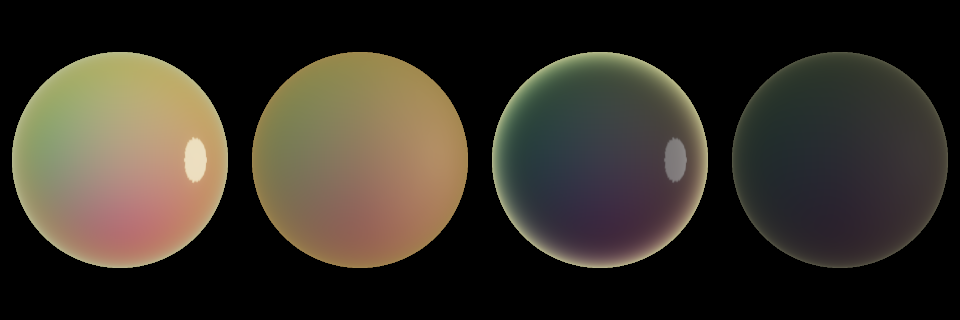
\includegraphics[width=.89\linewidth]{../../../output/profiling/environment-lighting/material-spheres.png}
\caption{Redflag 的 Vulkan 着色器绘制的镜面反射。四个球依次为光滑金属、粗糙金属、光滑涂漆、粗糙涂漆，使用同一张带亮窗的测试全景。球的形状和底色相同。}
\end{figure}

光滑表面主要映出 $R$ 附近很小一片天空。粗糙表面有许多朝向稍有不同的小面，同一条视线会收到更大一片环境的光。从左向右看图中前两颗球，亮窗的轮廓展开，最亮处也变暗了。我们可以预先把不同方向附近的光做加权平均，保存五层倒影。第 0 层保留细节，第 4 层反射范围最宽。粗糙度为 $0.375$ 时，着色器取第 $4\times0.375=1.5$ 层，即把第 1、2 层各取一半。五层是本项目的存储选择。

环境给出了光从哪里来，还要估计表面把多少光反射回来。光正对空气和普通玻璃的交界面时，按折射率 $1$ 与 $1.5$ 计算，反射比例约为 $((1.5-1)/(1.5+1))^2=0.04$。这里把它作为普通非金属的起点。纯金属则用材质底色描述正面反射的颜色。实现根据观察角度和粗糙度查一张预先积分的二维表。表里有两个系数，用来把环境的颜色换算成表面朝观察者反射的亮度。
\readings{\href{https://www.pbr-book.org/4ed/Reflection_Models/Roughness_Using_Microfacet_Theory}{PBRT 第四版 §9.6，微表面}\quad\href{https://learnopengl.com/PBR/IBL/Specular-IBL}{LearnOpenGL，Specular IBL}\quad\src{Redflag/src/Redflag/Renderer/ScreenSpace/Shaders/Environment.glsl}{Environment.glsl}}

\clearpage
\section{屏幕内外的倒影}
摄影棚的机身右侧有一道窄边。固定镜头和灯，只切换“镜面 IBL”，两张图里这道边受到的光便有明显差别。底色、法线和两项材质参数来自同一件模型。两次截帧中用于照明的底色和材质图逐像素相同。

\newcommand{\studioview}[2]{\begin{minipage}{.485\linewidth}\centering
\begin{tikzpicture}
  \node[inner sep=0,anchor=south west] (shot) at (0,0) {\includegraphics[width=\linewidth]{../../../output/profiling/material-studio/#1.png}};
  \begin{scope}[x={(shot.south east)},y={(shot.north west)}]
    \draw[white,line width=.9pt] (.6556,.5702) circle[radius=1.6mm];
    \draw[black,line width=.25pt] (.6556,.5702) circle[radius=1.8mm];
  \end{scope}
\end{tikzpicture}\\\small #2\end{minipage}}
\begin{figure}[H]\centering
\studioview{no-ibl}{关闭镜面 IBL}\hfill\studioview{after}{开启镜面 IBL}
\caption{Khronos 示例 Antique Camera 和 Poly Haven 全景 Studio Small 09。白圈中心是机身边框上的像素 $(524,220)$。取它周围 $5\times5$ 个像素，在显示变换前读回线性红通道，平均值从 0.00524 升到 0.24281。}
\end{figure}

在组合光照中，\code{LightingPreview::RenderLit} 先准备直接光和漫反射的颜色。若场景选了环境图，就可以再加上镜面看到的环境。打开屏幕空间反射（SSR）后，反射光线有时会先碰到画面里的一堵墙。这时应该用墙的颜色。走出屏幕或找不到合适的交点时，环境仍能提供来自该方向的光。下面是两条路在着色器里的简写。

\begin{lstlisting}
// (*@伪代码。surfaceLighting 已包含直接光和间接漫反射。@*)
vec3 reflected = sampleEnvironment(R, roughness);
if (screenRayHitsWall)
    reflected = sampleWallLight() * reflectionWeight;
return surfaceLighting + reflected;
\end{lstlisting}
\noindent{\small 着色器见 \src{Redflag/src/Redflag/Renderer/ScreenSpace/Shaders/StochasticSSR.comp}{StochasticSSR.comp} 的 \code{main}。它调用 \code{specularEnvironment} 时，已经计入材质的反射比例。}

可以摆两片金属和一堵绿墙来检查。第一片能从屏幕里找到绿墙，开关镜面 IBL，像素的四个分量都相同。第二片向画外反射，开启后测得线性 RGB 为 $(1.717,0.511,0.120)$。这个实验能发现同一处倒影被加亮两次的问题。全景只记录了从一个位置看到的房间，若要还原紧靠物体、又藏在取景框外的遮挡，还需要该物体附近的几何信息。
\readings{\src{output/profiling/environment-lighting/README.md}{绿墙与画外反射的截帧}\quad\src{output/profiling/material-studio/measurements.json}{摄影棚的亮度读数}\quad\href{https://polyhaven.com/a/studio_small_09}{Sergej Majboroda，Studio Small 09}}
